\label{sec:testbed}

We proceed to define the testbed environment by each of its conforming
parts. We later indicate a procedure to set up the testbed. In this procedure,
we summarize all the details regarding on setting the connectivity and
system files for a set of \ac{Raspi}s in a decentralized and/or centralized fashion
depending on the testbed admins preferences..
%Afterwards, we indicate how to cross-compile C++ code and the Kodo
%network coding library in an easy way.
%Finally, we provide further information about Kodo itself in terms
%of testing, other platforms supported and source code documentation
%for further references.

\subsection{System Overview}


\begin{figure}[ht!]
\centering
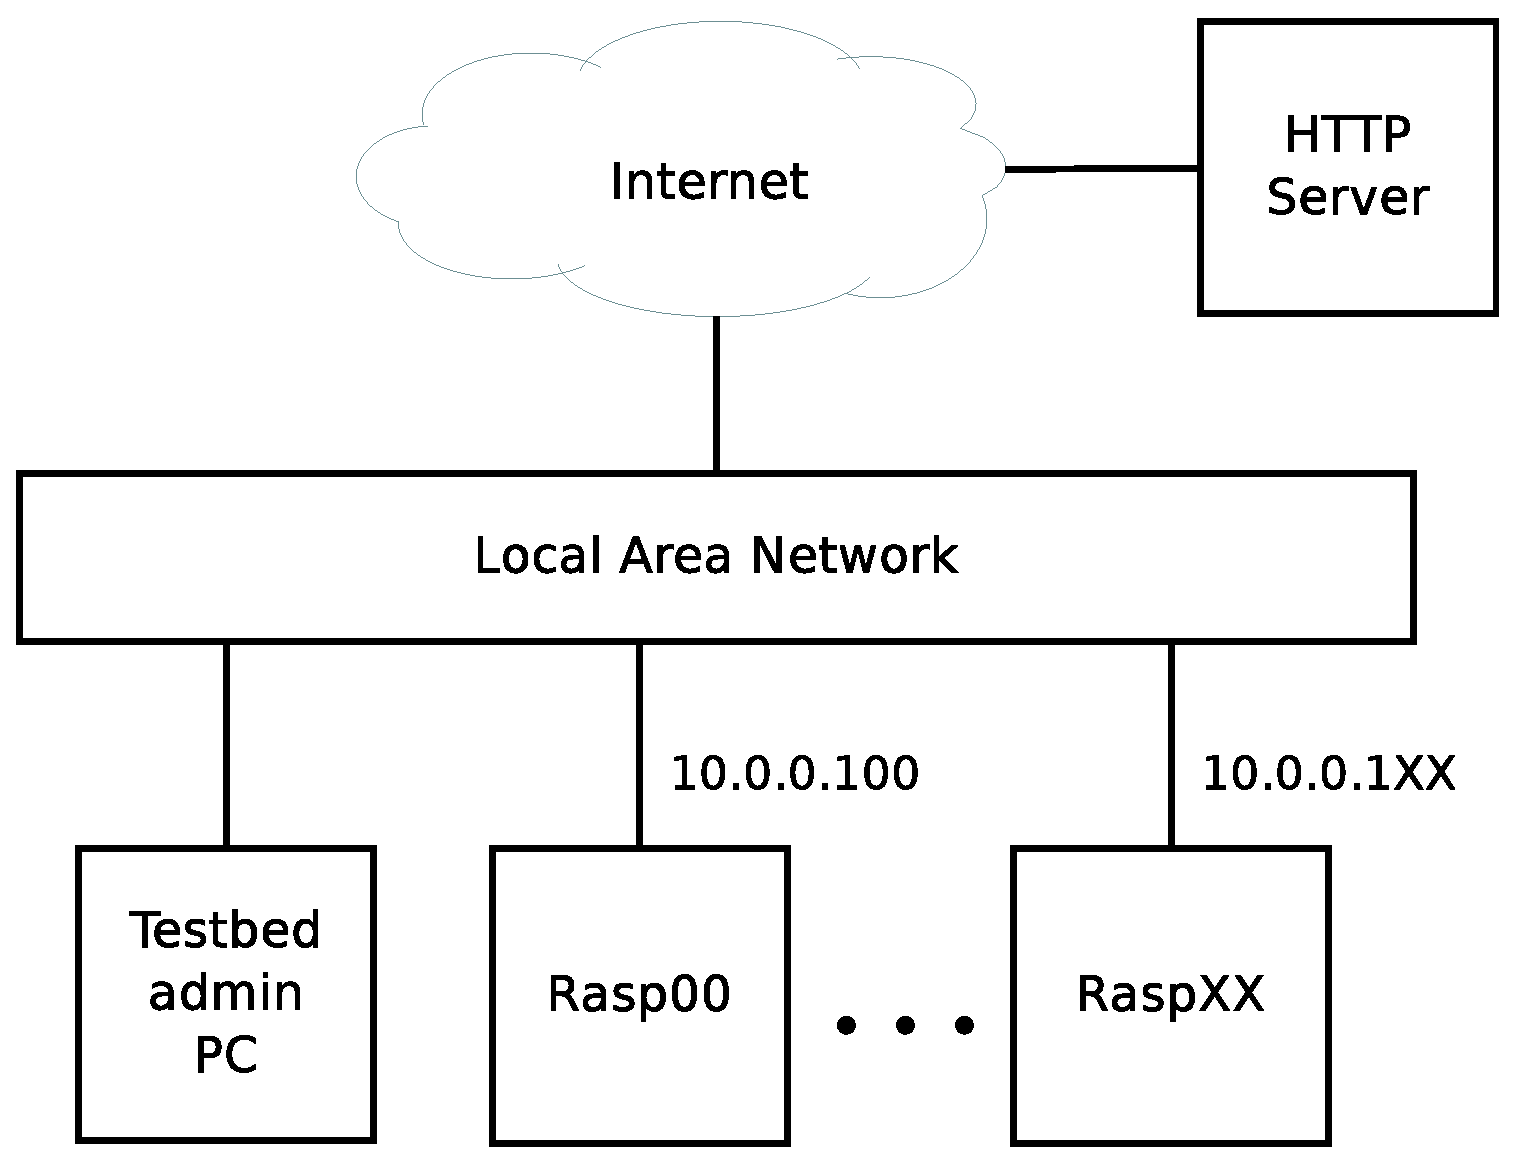
\includegraphics[width=0.45\textwidth]{images/testbed_setup3.eps}
\caption{Testbed setup}
\label{fig:testbed_setup}
\end{figure}

The testbed consists of up to one hundred \ac{Raspi}s of different models.
More specifically, Raspberry Pi 1 model B rev.~2,
Raspberry Pi 2 model B V1.1, and Raspberry Pi 3 model B V1.2.
All \ac{Raspi}s are each equipped with a memory card, a wired, and a wireless
network interface. They connect to the university network using its wired
ethernet interface that is named \texttt{eth0} according to the legacy naming
convention of ethernet interfaces in Linux~\cite{PredictableNetworkInterfaceNames}.

All \ac{Raspi}s will be running an \ac{SSH} daemon for easy remote access
within the university network. We therefore had the university's \ac{IT}
department configure the university's \ac{DHCP} server to assign each \ac{Raspi} a
static \ac{IP}. This eliminates the requirements for monitors and keyboards
for the \ac{Raspi}s for non-graphical applications.
%This significantly eases the management of the \ac{Raspi}s
%as \ac{SSH} eliminates the need for monitors and keyboards for the \ac{Raspi}s.

A sketch of the testbed is depicted in Figure~\ref{fig:testbed_setup}.
The testbed is intended for students to perform simulations and measurements
as part of semester projects. We therefore intend to configure all
\ac{Raspi}s identically, while still allowing students to alter how each
\ac{Raspi} behaves and is configured.

The following produre explains a way to setup the testbed to facilitates these
requirements. The procedure is assumed to be performed by whom we will refer
to as the testbed administrator in a \ac{PC} running Linux. The exact Linux
distribution is does not matter, but the procedure will be based on
Debian Linux.





The testbed should be available for students to perform simulations and
measurements as part of their semester projects. We intend to configure
all \ac{Raspi}s identically, while still allowing students to alter
how each \ac{Raspi} behaves and is configured.

When working on the testbed with this many devices, it may not always be
desired to make persistent changes to devices. We present how the concept
of stacked filesystems may be used to enable the means of both persistent
and temporary storage.

%The testbed should be available for students to perform simulations and
%measurements as part of their semester projects. The \ac{Raspi}s should
%be configured identically, but allows the students to alter the
%configurations and how each \ac{Raspi} behaves.
%
%When working on a testbed with many devices, it may not always desired
%to make persistent changes to devices. We present how the concept of stacked
%filesystems may be used to enable the means of both persistent and
%temporary storage.

%A \ac{HTTP} server will be used to store Linux configuration files as well
%as the root filesystem in the centralized approach.





The following procedure explains how the testbed may be setup and configured.

%The following procedure will explain how the testbed may be setup and
%configured both in the traditional distributed fasion where the
%entire Linux filesystem is written to an memory card, but also in a more
%centralized fasion where 
%is written to
%Based on the popular Debian based Raspbian Linux distribution
%We
%first present how a standard Linux distribution for the \ac{Raspi}s
%may be customized 


\subsubsection{Installing Raspbian}

To get started, we first need to install an \ac{OS} on the
\ac{Raspi}s. We will use the popular Debian-based Raspbian
Linux~\cite{raspbian}

We will be using a \ac{PC} running a Debian-based Linux distribution
to setup a customized Raspbian Linux image that can be written to
a memory card and work in any \ac{Raspi} version 1 or 2.

Raspbian is made available in two bundles: Raspbian and Raspbian lite.
The difference between the two is that Raspbian contains a pre-installed desktop
environment, and Raspbian lite is by default only accessible through a 
command shell. Both Raspbian and Raspbian lite will both by default be remotely
accessible using \ac{SSH}. \ac{SSH} provides the means to remotely
connect to another machine through a command shell.
%In fact it is the successor
%of \ac{Telnet} that has been designed with network security in mind.

The \ac{Raspi}s in our testbed is not connected to monitors, so we
have decided to go with Raspbian lite.
%Our testbed does not have monitors so we will install Raspbian lite.
A desktop environment can be installed using the package manager
(apt-get) in case a desktop environment will be desired at a later
time.

Below is the procedure we followed to setup the \ac{Raspi}s in our testbed. We
have performed a simple setup where each \ac{Raspi} is equipped with a
memory card that contains a slightly customized Raspbian lite image. The image
of the \ac{OS} in all \ac{Raspi}s will be identical.

The overall procedure to customize the official Raspbian lite image
are:
\begin{enumerate}
    \item Download Raspbian lite
    \item Alter Raspbian lite. e.g. browse, modify, add, and delete files
        in the official Raspbian lite image
    \item Change root, i.e. change root filesystem into the Raspbian lite
        image to update and install software packages
    \item Write image to memory cards
\end{enumerate}

Hashmark (\#) and dollar (\$) will be used throughout the code blocks in
the paper to indicate if an operation needs to be run with root permissions or
user permissions.

\subsection{Download Raspbian lite}

The latest Raspbian lite image can be downloaded at~\cite{raspbian}.
%To download the latest Raspbian lite, we go to the url
%\url{http://downloads.raspberrypi.org/raspbian_lite/images/}.
At the time of this writing, the latest bundle was
2016-05-27-raspbian-jessie-lite.zip.

we want to proceed downloading the image in a shell instead of the browser.
to do this, first open a command shell on a linux machine. this guide is
assuming a debian-based distribution, but there should only be minor differences
if you have another package manager. i.e. the package managers and name of software packages.

After the terminal has been opened, we start by declaring a few variables to reduce
repeated typing. The first variables we declare is the Raspbian image name.
Notice that the extension has been omitted. This is because the image has been
packed into a zip file. The other variable we declare is a working directory.
This is where we will download the image to and work on it. In other words, it
will be stored in \texttt{/home/<username>/Raspbian}

%To download Raspbian lite, we go to the \url{http://downloads.raspberrypi.org}.
%There should be a folder called raspbian\lite and
%to find the download page at which Raspbian lite should be located. Instead of
%downloading with the browser, we just extract the download url to the latest
%image. At the time of this writing, that was

% Define variable]
\begin{lstlisting}[]
$ export IMAGE="2016-05-27-raspbian-jessie-lite"
$ export WORKDIR="${HOME}/Raspbian"
\end{lstlisting}
\FloatBarrier
\vspace{-5mm}

A final thing to notice is the way \$ and \# are used in the code blocks. \$
means that the command can be run with normal user permissions where \# indicates that the
command needs root permissions.
Running a command with root permissions can on most systems be done by putting
the command "sudo" in front of each line. This is illustrated in the code below
with the command "whoami" that prints the username of the caller. Lines without
leading \$ or \# is the terminal output.

% Root example
\begin{lstlisting}[]
$ whoami
<USERNAME>
$ sudo whoami
root
\end{lstlisting}
\FloatBarrier
\vspace{-5mm}

Next, we make the working directory and change directory (cd) into the working
directory. We can then use wget to download Raspbian lite. Unpack the image
when the download is complete.

% Download and unpack image
\begin{lstlisting}[]
$ mkdir -p ${WORKDIR}
$ cd ${WORKDIR}
$ wget http://kom.aau.dk/project/TuneSCode/raspi/${IMAGE}.zip
$ unzip ${IMAGE}.zip
\end{lstlisting}
\FloatBarrier
\vspace{-5mm}

A more recent version of Raspbian lite may be available at~\cite{raspbian}.
%\url{http://downloads.raspberrypi.org/raspbian_lite/images}.

\subsection{The image}

After Raspbian lite has been unpacked, there should be an .img file in the directory.
"fdisk" can be used to display the content of the image. Pass the arguments "-u sectors" to
display the sizes in sectors and "-l" to display partitions and automatically
exit fdisk again.

% Check out the image   % The dollar hack was to fix vim syntax
\begin{lstlisting}[literate={DOLLAR}{\$}1]
DOLLAR fdisk -u sectors -l ${IMAGE}.img
Disk 2016-05-27-raspbian-jessie-lite.img: 1.3 GiB, 1387266048 bytes, 2709504 sectors
Units: sectors of 1 * 512 = 512 bytes
Sector size (logical/physical): 512 bytes / 512 bytes
I/O size (minimum/optimal): 512 bytes / 512 bytes
Disklabel type: dos
Disk identifier: 0x6fcf21f3

Device                               Boot  Start     End Sectors  Size Id Type
2016-05-27-raspbian-jessie-lite.img1        8192  137215  129024   63M  c W95 FAT32 (LBA)
2016-05-27-raspbian-jessie-lite.img2      137216 2709503 2572288  1.2G 83 Linux
\end{lstlisting}
\FloatBarrier

The image is in total 2709504 sectors (1.3GiB) in size and contains two
partitions. The first partition starts at sector 8192 and
the other partition starts at sector 137216. The partitions is of type FAT32
and Linux and have sizes 63M and 1.2G. This indicates that the first partition
is most likely a boot partition and the second partition is a traditional Linux file
system. Actually, it is the Linux root filesystem (i.e. /).

\subsection{Resize image}
1.2G is not very much to hold the root filesystem given that it is desired to
in later steps alter the files and install more packages. It may therefore be
necessary to increase the partition size slightly.
The following steps illustrates how the image and its root filesystem
can be expanded by one \ac{GB}.

First, expand the image one \ac{GB} and wait for the data to be completely written
to the disk:
\begin{lstlisting}[]
$ dd if=/dev/zero bs=1M count=1024 >> ${IMAGE}.img && sync
\end{lstlisting}
\FloatBarrier
\vspace{-5mm}

Use \texttt{fdisk} to check that the image is one \ac{GB} bigger:
\begin{lstlisting}[literate={DOLLAR}{\$}1]
DOLLAR fdisk -u sectors -l ${IMAGE}.img
Disk 2016-05-27-raspbian-jessie-lite.img: 2.3 GiB, 2461007872 bytes, 4806656 sectors
Units: sectors of 1 * 512 = 512 bytes
Sector size (logical/physical): 512 bytes / 512 bytes
I/O size (minimum/optimal): 512 bytes / 512 bytes
Disklabel type: dos
Disk identifier: 0x6fcf21f3

Device                               Boot  Start     End Sectors  Size Id Type
2016-05-27-raspbian-jessie-lite.img1        8192  137215  129024   63M  c W95 FAT32 (LBA)
2016-05-27-raspbian-jessie-lite.img2      137216 2709503 2572288  1.2G 83 Linux
\end{lstlisting}
\FloatBarrier
\vspace{-5mm}

Now, to expand the root filesystem it is required to first remove the Linux partition
and then add it again one \ac{GB} bigger.
We use \texttt{fdisk} to alter the partition table. The echo's within the parenthesis
will function as
key-presses in \texttt{fdisk} and hence delete last partition, create a new
primary partition, print new partition table, and write new partition table
to the image:

\begin{lstlisting}[]
$ (echo d; echo ; echo n; echo p; echo ; echo 137216; echo ; echo p; echo w) | fdisk ${IMAGE}.img
\end{lstlisting}
\FloatBarrier
\vspace{-5mm}

Use a loopback device to make the Raspbian image available as a block device: 
\begin{lstlisting}[]
# export DEV=$(sudo losetup --show -f -P ${IMAGE}.img); echo $DEV
/dev/loop0
\end{lstlisting}
\FloatBarrier
\vspace{-5mm}

It is seen that the image is now available as \texttt{/dev/loop0}. Use \texttt{lsblk}
to view the partitions:

\begin{lstlisting}[]
# lsblk
NAME      MAJ:MIN RM  SIZE RO TYPE MOUNTPOINT
...
loop0       7:0    0  2.3G  0 loop 
|-loop0p1 259:2    0   63M  0 loop 
|-loop0p2 259:3    0  2.2G  0 loop
...
\end{lstlisting}
\FloatBarrier
\vspace{-5mm}

Check and resize the root partition:
\begin{lstlisting}[]
# e2fsck -f ${DEV}p2
# resize2fs ${DEV}p2
\end{lstlisting}
\FloatBarrier


%We see that the boot and root partitions starts at sector 8192 and 137216 respectivly.
%We also notice that each sector is 512 bytes.
%On newer systems, we can mount the device easier using "losetup --show -f -P IMAGE"
%Mount root partition:

\subsection{Mount image}

Browsing and altering the files in the image is easy. Simply mount the partitions.
%To browser and alter the files in the image, it is possible to mount the partitions.

Lets first mount the root partition. This is done by creating an empty directory
that we will be used as a mountpoint. We name it \texttt{root} and create it in the
working directory.
After this, simply mount the partitions:
%After this,
%we mount the partition starting at sector 137216. To provide this offset information
%to mount, we need to find the offset in bytes. From the fdisk command we could also
%see that each sector is 512 bytes. Thus, we multiply the sector size and the sector
%start to get the offset in bytes.

\begin{lstlisting}[]
$ export ROOTDIR="${WORKDIR}/root"
$ mkdir -p ${ROOTDIR}
# mount ${DEV}p2 ${ROOTDIR}
\end{lstlisting}
\FloatBarrier
\vspace{-5mm}
%# mount -o loop,offset=$((137216*512)) ${IMAGE}.img ${ROOTDIR}

After this, we can also mount the boot partition inside the newly mounted
root filesystem. This is convenient because that partition will be mounted
on this directory when a \ac{Raspi} starts up with a memory card containing
the image. %It is therefore the natural place to mount it for later purposes.

Mount boot partition:
\begin{lstlisting}[]
# mount ${DEV}p1 ${ROOTDIR}/boot
\end{lstlisting}
\FloatBarrier
\vspace{-5mm}
%# mount -o loop,offset=$((8192*512)) ${IMAGE}.img ${ROOTDIR}/boot

We can now change all the files in the disk image as desired.



\subsection{Configuring OS files and scripts}

The \ac{Raspi}s should be setup as similar as possible. One of those
few settings that may be different in the devices is their hostname that
helps the user to distinguish the devices from each other.
%The hostname helps distinguish them from each other.
One approach to create unique hostnames would be to rename the hostname
in each memory card. Another way is to create a start up script to automatically
configure the hostname. We decided to define the hostnames based on the \ac{MAC}
addresses of the \ac{Raspi}s wired ethernet interface.

%The \ac{Raspi}s should be setup to be as similar as possible. One of those
%things that is preferred to be different on the devices is their hostname.
%This helps distinguish them from each other. One solution to this in our
%approach would be to uniquely change the hostname in each memory card.
%This is however not desired because that would either require modifying
%the customized Raspbian lite image before writing the content to the
%memory card or to manually change it in the \ac{Raspi}s after the image has
%been written to a memory card.
%Instead, we decided to register the ethernet MAC addresses of all the \ac{Raspi}s
%in our testbed. Those had to be used to put them in a domain name anyway.
%
%Below is a part of the file where we keep track of the MAC addresses and assign
%hostnames. This file will be available online and copied to the Raspbian lite
%image in a later step under the listed filename. For different \ac{Raspi}s
%the MAC addresses has to be changed. The MAC address of a network card can be found
%using the command \texttt{"ifconfig"} or \texttt{"ip addr"}.

%Instead, we decided to register the ethernet MAC addresses of all the \ac{Raspi}s
%in our testbed. Those had to be used to put them in a domain name anyway.

Below is a snippet of the file of all the hostnames and \ac{MAC} addresses:

%Below is a part of the file where we keep track of the MAC addresses and assign
%hostnames.
%This file will be available online and copied to the Raspbian lite
%image in a later step under the listed filename. For different \ac{Raspi}s
%the MAC addresses has to be changed. The MAC address of a network card can be found
%using the command \texttt{"ifconfig"} or \texttt{"ip addr"}.


% MAC and Hostname file
\Suppressnumber\begin{lstlisting}[]
<@\textcolor{gray}{\$\{ROOTDIR\}/home/pi/rasp\_config/nodes.csv}@>
<@\textcolor{gray}{
---------------------------------------------------------------}
\Reactivatenumber @>
# Ethernet MAC    Hostname
b8:27:eb:5b:da:20 rasp00
b8:27:eb:7b:c3:91 rasp01
b8:27:eb:54:9c:64 rasp02
b8:27:eb:95:bd:11 rasp03
\end{lstlisting}
\FloatBarrier
\vspace{-5mm}

%Provided that each \ac{Raspi} will have knowledge of all other \ac{Raspi}s in
%the testbed, it still needs to know which name to give itself.
%We do this using a small Bash script:
We use the \ac{Bash} script below to enable each \ac{Raspi} to find its
hostname in \texttt{nodes.csv}.

% Set hostname
\Suppressnumber\begin{lstlisting}[]
<@\textcolor{gray}{\$\{ROOTDIR\}/home/pi/rasp\_config/set\_hostname}@>
<@\textcolor{gray}{
---------------------------------------------------------------}
\Reactivatenumber @>
#!/usr/bin/env bash

script_path="$(dirname $(realpath $0))"
config_file=${script_path}/nodes.csv 
mac=$(cat /sys/class/net/eth0/address)
old_hostname=$(hostname)
new_hostname=$(grep $mac $config_file | cut -f2 -d' ')

# Assign hostname found in nodes.csv
if [ ! -z ${new_hostname} ]; then
    echo ${new_hostname} > /etc/hostname
    hostname ${new_hostname}
    sed -i.old -e "s:${old_hostname}:${new_hostname}:g" /etc/hosts
fi
\end{lstlisting}
\FloatBarrier
\vspace{-5mm}

Line 1 tells the system to interpret the script using Bash. Line 3 gets the
path of the script itself. Line 4 gets the MAC address. This script will be
located in all \ac{Raspi}s and thus return the MAC address of the node itself
when executed.
Line 4 searches line by line for this mac address.
Line 8-11 assigns the hostname found in \texttt{"nodes.csv"}. If the MAC did not exists,
then it will keep the default hostname of the system.

It is likely that the testbed administrator needs to either change or add
scripts to configure the \ac{Raspi}s. This would be tedious to distribute to
all \ac{Raspi}s. One way around this is to make the \ac{Raspi}s fetch the
configuration scripts during start up before running the configuration scripts.

The below script attempts to fetch the scripts:

\Suppressnumber\begin{lstlisting}[]
<@\textcolor{gray}{\$\{ROOTDIR\}/home/pi/rasp\_config/update\_rasp\_config}@>
<@\textcolor{gray}{
---------------------------------------------------------------}
\Reactivatenumber @>
#!/usr/bin/env bash

url="http://kom.aau.dk/project/TuneSCode/raspi/"
config_file="rasp_config.zip"

# Attempt to fetch new configuration files
if ! wget -O -q --show-progress /tmp/${config_file} ${url%/}/${config_file}; then
    echo "Warning: Unable to update rasp_config files"
    exit 1
fi

# Unzip and overwrite configurationn files to root's home directory
unzip -q -o /tmp/${config_file} -d /home/pi/
\end{lstlisting}
\FloatBarrier
\vspace{-5mm}


We have packed the files and uploaded them to a webserver. These can be
retrieved with \texttt{wget} and unzipped into the Raspbian lite image that
we are customizing:

% Get the files
\begin{lstlisting}[]
$ wget http://kom.aau.dk/project/TuneSCode/raspi/rasp_config.zip
$ unzip rasp_config.zip -d ${ROOTDIR}/home/pi/
\end{lstlisting}
\FloatBarrier
\vspace{-5mm}

For the above to work in the \ac{Raspi}s, it is required that the \ac{Raspi}
\ac{MAC} address is found in \texttt{nodes.csv}. Thus,
\texttt{rasp\_config.csv} needs to be unzipped, altered, and zipped again in
the http server from which the \ac{Raspi} retrieves the files from.
%"nodes.csv" can be changed using a text editor. For vim, this could be done
%the following way:
%\begin{lstlisting}[]
%$ vim ${ROOTDIR}/home/pi/rasp_config/nodes.csv
%\end{lstlisting}
%\FloatBarrier
%\vspace{-5mm}


Finally, to actually make the \ac{Raspi}s change hostname, we have to make
each \ac{Raspi} call the above script when it starts up. Optionally,
also run the update script before running other scripts.
Do this with root permissions by inserting the line below before
\texttt{"exit 0"} using your favorite editor:
%"\$\{ROOTDIR\}/etc/rc.local" using
%your favorite text editor..
%The file
%can be opened with your favorite text editor.

\Suppressnumber\begin{lstlisting}[]
<@\textcolor{gray}{\$\{ROOTDIR\}/etc/rc.local}@>
<@\textcolor{gray}{
-----------------------------------------------------}
\Reactivatenumber @>
...
bash /home/pi/rasp_config/update_rasp_config
bash /home/pi/rasp_config/set_hostname
...
exit 0
\end{lstlisting}
\FloatBarrier
\vspace{-5mm}

Configuring \texttt{rc.local} makes it really cumbersome for the testbed
administrator to add new scripts since a new script first needs to be added
in \texttt{rasp\_config.zip} and then run by adding an additional line of code
to \texttt{rc.local} in the root image or in all memory cards depending on
the final testbed setup.

A solution to this is to have yet another script in \texttt{rasp\_config.zip}
that calls all the other scripts in the desired order. This would look like
below:
\Suppressnumber\begin{lstlisting}[]
<@\textcolor{gray}{\$\{ROOTDIR\}/home/pi/rasp\_config/main}@>
<@\textcolor{gray}{
-----------------------------------------------------}
\Reactivatenumber @>
#!/usr/bin/env bash

bash /home/pi/rasp_config/set_hostname
\end{lstlisting}
\FloatBarrier
\vspace{-5mm}

Now, to use the above script, it is required to change \texttt{rc.local}
slightly:
\Suppressnumber\begin{lstlisting}[]
<@\textcolor{gray}{\$\{ROOTDIR\}/etc/rc.local}@>
<@\textcolor{gray}{
-----------------------------------------------------}
\Reactivatenumber @>
...
bash /home/pi/rasp_config/update_rasp_config
bash /home/pi/rasp_config/main
...
exit 0
\end{lstlisting}
\FloatBarrier
\vspace{-5mm}
Notice that \texttt{set\_hostname} is now called through the \texttt{main}
script instead. The update script is still called directly. This ensures that
all configuration scripts are updated before executed. Changes to the update
script itself will first take effect at system startup. Had the update script
been called in \texttt{main} instead would mean that changes to the 
\texttt{main} script would also first have been available at next startup.

%This can be done by inserting a call to the script
%set\_hostname in rc.local before it exits.
%
%Call set\_hostname script at startup. We insert a line of code to call script in rc.local just after the initial comments (i.e. lines starting with \#).
%\begin{lstlisting}[]
%# line_number=$(egrep -n -m1 "(^[^#])|(^$)" ${ROOTDIR}/etc/rc.local | cut -d: -f1)
%# sed -i "${line_number}c bash /home/pi/rasp_config/set_hostname" ${ROOTDIR}/etc/rc.local
%\end{lstlisting}
%\FloatBarrier
%$ line="bash /home/pi/.rasp_config/set_hostname"
%# awk -v text="$line" '!/^#/ && !p {print text; p=1} 1' ${ROOTDIR}/etc/rc.local > <@ \Suppressnumber @>
%    ${ROOTDIR}/etc/rc.local <@ \Reactivatenumber @>

WE NEED TO ADD A FEW COMMANDS TELLING HOW TO ZIP, MODIFY, AND UNZIP
FOR THE READER TO BE ABLE TO UPLOAD A CONSTRUCT HIS/HER OWN BUNDLE.

All other files could be updated as well.

\subsection{Installing and updating the image}

It may be desired to pre-install some programs in the image before it is
written to all the memory cards that goes into the \ac{Raspi}s.
This can be done from any linux x86 machine using QEMU Chroot~\cite{QemuUserEmulation}
(change root).
%\url{https://wiki.debian.org/QemuUserEmulation}
%\url{https://wiki.archlinux.org/index.php/Raspberry_Pi}

Due to the \ac{ARM} processor that \ac{Raspi}s are using, it is required to
install some additional software:
%Because \ac{Raspi}s are equipped with an \ac{ARM} processor 
%%it is not as
%straightforward as performing the task for two Linux systems of the same
%architecture.

% CHROOT to OS image
\begin{lstlisting}[]
# apt-get install binfmt-support qemu qemu-user-static
# update-binfmts --display qemu-arm
qemu-arm (enabled):
     package = qemu-user-static
        type = magic
      offset = 0
       magic = \x7fELF\x01\x01\x01\x00\x00\x00\x00\x00\x00\x00\x00\x00\x02\x00\x28\x00
        mask = \xff\xff\xff\xff\xff\xff\xff\x00\xff\xff\xff\xff\xff\xff\xff\xff\xfe\xff\xff\xff
 interpreter = /usr/bin/qemu-arm-static
    detector = 
\end{lstlisting}
\FloatBarrier
\vspace{-5mm}
% This was neccessary on arch
%# update-binfmts --importdir /var/lib/binfmts/ --import

Make sure the second command writes "enabled" as the output above. If that 
is not the case, then try enabling it:

\begin{lstlisting}[]
# update-binfmts --enable qemu-arm
\end{lstlisting}
\FloatBarrier
\vspace{-5mm}

Provided that qemu-arm is enabled, we should now be able to change root (chroot)
into our Raspbian lite image. Change root is a method i linux that enables
the root (/) to be changed. Thus, enabling a linux installation within a
linux installation.

There are a few commands to be performed before we can change root.
First, to get internet access from within the Raspbian lite image it is needed
to copy our resolv.conf into the filesystem. Line 1 steps into Raspbian lite's
root filesystem. Then line 2 copies resolv.conf.

% CHROOT to OS image
\begin{lstlisting}[]
$ cd $ROOTDIR
# cp /etc/resolv.conf ${ROOTDIR}/etc/resolv.conf
\end{lstlisting}
\FloatBarrier
\vspace{-5mm}

Now, because of the ARM architecture, it is also required to copy
/usr/bin/qemu-arm-static into the image before we can continue:

% CHROOT to OS image
\begin{lstlisting}[]
# cp /usr/bin/qemu-arm-static ${ROOTDIR}/usr/bin
\end{lstlisting}
\FloatBarrier
\vspace{-5mm}

The final preparation before chaning root is to populate the directories proc,
sys, and dev:

% CHROOT to OS image
\begin{lstlisting}[]
# mount  -t proc proc proc/
# mount --bind /sys sys/
# mount --bind /dev dev/
# mount --bind /dev/pts dev/pts
\end{lstlisting}
\FloatBarrier
\vspace{-5mm}

Finally, the filesystem is ready for us to change root. This can be done with
"proot". It may be required to install proot:

% CHROOT to OS image
\begin{lstlisting}[]
# proot -q qemu-arm-static -S ${ROOTDIR}
\end{lstlisting}
\FloatBarrier
\vspace{-5mm}

Most available online material uses the more known chroot command as written in
the code block below. This did not work correctly in our machines, but we show
it as an alternative in case proot may not work on other systems.

% CHROOT to OS image
\begin{lstlisting}[]
# chroot ${ROOTDIR} /usr/bin/qemu-arm-static /bin/bash    (ALTERNATIVE TO proot)
\end{lstlisting}
\FloatBarrier
\vspace{-5mm}

If everything went well, we should now be standing in the Raspbian lite filesystem
under its root. Optionally, we can change the prompt title to indicate that we
are chrooted:

% Optionally, we may create a unique prompt to indicate we have changed root
\begin{lstlisting}[]
# export PS1="(chroot) $PS1"
\end{lstlisting}
\FloatBarrier
\vspace{-5mm}

The Raspbian lite system should now be possible to use as if it had been booted
in a \ac{Raspi}. The only difference is that the laptop that we are using is
significantly faster than a \ac{Raspi}. Thus enabling us to for example update,
upgrade, and install software packages:

% Update system
\begin{lstlisting}[]
(chroot) # apt-get update
(chroot) # apt-get upgrade
\end{lstlisting}
\FloatBarrier
\vspace{-5mm}

Lets install some useful applications:
% Install packages
\begin{lstlisting}[]
(chroot) # apt-get install vim git screen
\end{lstlisting}
\FloatBarrier
\vspace{-5mm}

All the changes that are made here will exists in all \ac{Raspi}s when the
image is written to a memory card.

\subsection{Installation an overlaying filesystem}

Our goal was to enable the users of the testbed to change however the
\ac{Raspi} are configured while still being able to revert those changes easily.

We do this by storing a users work in the \ac{Raspi}s in \ac{RAM}. Thus a
\ac{Raspi}, when a \ac{Raspi} is rebooted, it will forget all changes.

A way to do this is using stacked filesystem. Stacking filesystem enables
a filesystem to overlay another filesystem. Whenever a file is accessed,
the upper filesystem will forward the request to the lower filesystem in
case it does not have it itself. If it has it, it will simpy return the file.

This idea can be used in our setup to mount the root filesystem (i.e. Raspbian
lite) in the \ac{Raspi}s duing startup as read-only. Thus, the files will not
be changable. Some programs needs to change files and the testbed admin might
want to change configurations. To enable this, it is possible to
overlay a filesystem that is mounted in \ac{RAM} as read/writable on top of
the regular root. Thus, reading a file may return a file from the lower filesytem,
but if it is stored, it will be saved in the upper filesystem. Accessing this file
again will return the stored file from the upper layer.



%We do this using an overlay filesystem. The idea is to let the \ac{Raspi}s
%mount their root filesystem as 
%
%We do this using an overlay filesystem (overlayfs).
%Overlayfs enables a filesystem to be stacked on top of another filesystem. Thus,
%if the \ac{Raspi}s mount their root filesystem (/) as read-onlyif we mount our root (/) filesystem as 
%
%
%Overlayfs enables filesystems
%to be stacked on top of each other. We will be using this to make a lower
%filesystem and an upper filesystem. The lower filesystem will be our
%traditional filesystem and the upper filesystem will be mounted in tmpfs
%(i.e. mounted in \ac{RAM}).
%
%Thus, when a file is requsted from stacked filesystem, it will first attempt
%to fetch the file in the upper filesystem if it does not exists there, it will
%request it from the lower filessytem.  

Assuming that you are still \texttt{chrooted} into the Raspbian lite filesystem, we
can setup the overlay filesystem (overlayfs).

There already exists implementations overlaying the root filesystem. We will
use an existing implementation
available at github: \cite{overlayroot}.

We installed git in a previous step, so lets clone the repository. The below
code stores it in /tmp which is really mounted in \ac{RAM}. Thus, the files
will disappear when the machine is rebooted.

% Get files
\begin{lstlisting}[]
(chroot) # OVERLAYROOTDIR="/tmp/overlayroot"
(chroot) # git clone https://github.com/chesty/overlayroot.git $OVERLAYROOTDIR
\end{lstlisting}
\FloatBarrier
\vspace{-5mm}

To enable the overlaying filesystem it is required to generate an initial \ac{RAM}
file system (initramfs). Initramfs is an initial filesystem that gets loaded into
\ac{RAM} during the startup process of a linux machine to prepare the real
filesystem.

For this purpose, we need BuxyBox:

% Install required packages
\begin{lstlisting}[]
(chroot) # apt-get install busybox
\end{lstlisting}
\FloatBarrier
\vspace{-5mm}

Add and activate the overlaying filesystem, we need to add the scripts and tell initramfs
to load the overlaying filesytem:

% Setup initramfs
\begin{lstlisting}[]
(chroot) # cp ${OVERLAYROOTDIR}/hooks-overlay /etc/initramfs-tools/hooks/
(chroot) # cp ${OVERLAYROOTDIR}/init-bottom-overlay /etc/initramfs-tools/scripts/init-bottom/
(chroot) # echo "overlay" > /etc/initramfs-tools/modules
\end{lstlisting}
\FloatBarrier
\vspace{-5mm}

%Finally, lets generate the initial \ac{RAM} filesystem. This is done using the command
%\texttt{mkinitramfs}, that will by default look for the kernel modules of the current system. Remember we are
%chrooted, so we need to specify the correct kernel modules to look for. These
%can be found in "/lib/modules".
Now, the initial \ac{RAM} filesystem can be generated. \ac{Raspi} version 1
needs a different kernel than \ac{Raspi} version 2 and version 3. Thus, start
by finding the available kernel modules:
%Because \texttt{initramfs} is executed within a
%\texttt{chrooted} environment, it will not be able to detect the
%kernel modules in the \texttt{chrooted} environment. The kernel modules will 


% Create an initramfs
\begin{lstlisting}[]
(chroot) # ls /lib/modules/
4.4.13+  4.4.13-v7+
\end{lstlisting}
\FloatBarrier
\vspace{-5mm}

Kernel "4.4.13+" is for \ac{Raspi} version 1 and kernel "4.4.13-v7+" works
for \ac{Raspi} version 2 and version 3.

Lets proceed by generating an initial \ac{RAM} filesystem for both kernels:

%Lets proceed with kernel modules "4.4.13+".
%Lets create an initial ram filesystem for both kernels.

%Thus, to run mkinitramfs, type in the correct kernel version:

% Create an initramfs
\begin{lstlisting}[]
(chroot) # mkinitramfs -o /boot/init.gz -k 4.4.13+
(chroot) # mkinitramfs -o /boot/init-v7.gz -k 4.4.13-v7+
\end{lstlisting}
\FloatBarrier
\vspace{-5mm}

%IT SEEM THAT THE RASPIS DEMANDS DIFFERENT KERNEL MODULES AFTER ALL.
%RASP-VERSION1=4.4.13+, RASP-VERSION2=4.4.13-V7+, RASP-VERSION3=4.4.13-V7+

Although there might be printet a few warnings, the above commands should successfully
generate working initial \ac{RAM} filesystems. 

An initial \ac{RAM} filesystem needs to be called by the bootloader. In Raspbian
this is done by adding a command to \texttt{config.txt} in the boot partition.

If the system should be run in a \ac{Raspi} version 1, then use \texttt{init.gz}:
%The bootloader should be made aware of the initramfs that we will generate:
\begin{lstlisting}[]
(chroot) # echo "initramfs init.gz" >> /boot/config.txt     # Only for Raspberry Pi version 1
\end{lstlisting}
\FloatBarrier
\vspace{-5mm}

If the system should be run in a \ac{Raspi} version 2 or 3, then use \texttt{init-v7.gz}:
\begin{lstlisting}[]
(chroot) # echo "initramfs init-v7.gz" >> /boot/config.txt  # Only for Raspberry Pi version 2 and 3
\end{lstlisting}
\FloatBarrier
\vspace{-5mm}

At this point, it is no longer required to be \texttt{chrooted} and the image
can be written to a memory card. The following commands exits the \texttt{chrooted}
environment, unmount all partitions, and detaches the loopback device:

% Exit chroot, umount, and write to memory card
\begin{lstlisting}[]
(chroot) # exit
# cd ..
# umount --recursive ${ROOTDIR}
# losetup -d ${DEV}
\end{lstlisting}
\FloatBarrier
\vspace{-5mm}

\subsection{(Optional) Persistent subdirectories for distributed Linux image}

EMPHASIZE THAT THIS SETUP IS ONLY FOR THE SETUP WHERE THE ROOT IMAGE ARE
WRITTEN TO THE MEMORY CARDS

Provided the stacked filesystem was configured, it may be desired to have
some directories where files are not flushed upon rebooting the \ac{Raspi}s.
The following procedure will create an extra partition in the image for
the \ac{Raspi} users home directory that will be made storage persistent.
%Provided that a stacked filesystem was configured to make the root
%filesystem forget chances upon reboots is not always desired. 

Expand image according to the desired home directory size. Keep in mind not
to make the image bigger than the target memory card.
% Expand image
\begin{lstlisting}[]
$ dd if=/dev/zero bs=1M count=1024 >> ${IMAGE}.img && sync
\end{lstlisting}
\FloatBarrier
\vspace{-5mm}

Create home partition after the root partition. Use \texttt{fdisk} to
find the next available sector in the image. In our case, the new
partition should start at sector 4806656:
\begin{lstlisting}[]
$ fdisk -lu ${IMAGE}.img
Disk 2016-05-27-raspbian-jessie-lite.img: 3.3 GiB, 3534749696 bytes, 6903808 sectors
Units: sectors of 1 * 512 = 512 bytes
Sector size (logical/physical): 512 bytes / 512 bytes
I/O size (minimum/optimal): 512 bytes / 512 bytes
Disklabel type: dos
Disk identifier: 0x6fcf21f3

Device                               Boot  Start     End Sectors  Size Id Type
2016-05-27-raspbian-jessie-lite.img1        8192  137215  129024   63M  c W95 FAT32 (LBA)
2016-05-27-raspbian-jessie-lite.img2      137216 4806655 4669440  2.2G 83 Linux
\end{lstlisting}
\FloatBarrier
\vspace{-5mm}

Create new partition:

\begin{lstlisting}[]
$ (echo n; echo p; echo ; echo 4806656; echo ; echo p; echo w) | fdisk ${IMAGE}.img
\end{lstlisting}
\FloatBarrier
\vspace{-5mm}

Create loopback device: 
\begin{lstlisting}[]
# export DEV=$(sudo losetup --show -f -P ${IMAGE}.img); echo $DEV
/dev/loop0
\end{lstlisting}
\FloatBarrier
\vspace{-5mm}

Format new partition:
\begin{lstlisting}[]
# mkfs.ext4 ${DEV}p3
\end{lstlisting}
\FloatBarrier
\vspace{-5mm}

The last thing to remember is to inform Raspbian to mount the home partition
we created during startup. This can be done by adding an entry in \texttt{fstab}:
\begin{lstlisting}[]
# mount ${DEV}p2 ${ROOTDIR}
# sudo sh -c "echo '/dev/mmcblk0p3 /home ext4 defaults,noatime 0 2' >> ${ROOTDIR}/etc/fstab"
\end{lstlisting}
\FloatBarrier
\vspace{-5mm}

The home folder was originally located in the root filesystem. We should
therefore copy the content to the new home partition:
\begin{lstlisting}[]
# mount ${DEV}p3 ${ROOTDIR}/mnt
# mv ${ROOTDIR}/home/* ${ROOTDIR}/mnt/
\end{lstlisting}
\FloatBarrier
\vspace{-5mm}

That is it. unmount partitions and detach loop device:
\begin{lstlisting}[]
# umount --recursive ${ROOTDIR}
# losetup -d ${DEV}
\end{lstlisting}
\FloatBarrier
\vspace{-5mm}

\subsection{Write image to memory card}


EMPHASIZE THAT THIS SETUP IS ONLY FOR THE SETUP WHERE THE ROOT IMAGE ARE
WRITTEN TO THE MEMORY CARDS

The final step is to write the image to all the memory cards before they can
be used in the \ac{Raspi}s.

%This is done by first leaving the \texttt{chrooted}
%filesystem and unmounting all the directories we mounted:

% Exit chroot, umount, and write to memory card
%\begin{lstlisting}[]
%# exit
%# cd ..
%# umount --recursive ${ROOTDIR}
%# losetup -d ${DEV}.img
%\end{lstlisting}
%\FloatBarrier
%\vspace{-5mm}

%If successfully unmounted, you can 
Insert a memory card in your machine. It will be available as
\texttt{/dev/mmcblkX} or \texttt{/dev/sdX}

%In most systems, this memory card was available under \texttt{/dev/mmcblk0}, but this may be
%different on different machines. For internal memory card readers, it will
%probably be named /dev/mmcblkX where X is some number and if the memory card
%reader is connected through \ac{USB}, then it is likely called /dev/sdX.
Make absolutely sure to write to the correct device as everything will be 
overwritten!
Inserting/Ejecting the memory card a couple of times and using the commands
below may help deducing the correct device:
%The commands below may help deduce which device is the correct:
%Below is a few commands that may help you to deduce which device is correct:

\begin{lstlisting}[]
# lsblk
# df -h
\end{lstlisting}
\FloatBarrier
\vspace{-5mm}

For us, the device was \texttt{/dev/mmcblk0}. Write the image to a memory card:
\begin{lstlisting}[]
# dd if=${IMAGE}.img of=/dev/mmcblk0 bs=4M && sync
\end{lstlisting}
\FloatBarrier
\vspace{-5mm}

The memory card can now be started in a \ac{Raspi}.

